% 16-exhibit-implementation
\begin{frame}[c]{Exhibit implementation}
\begin{columns}[T,onlytextwidth]
  \begin{column}{0.48\textwidth}
    \centering
    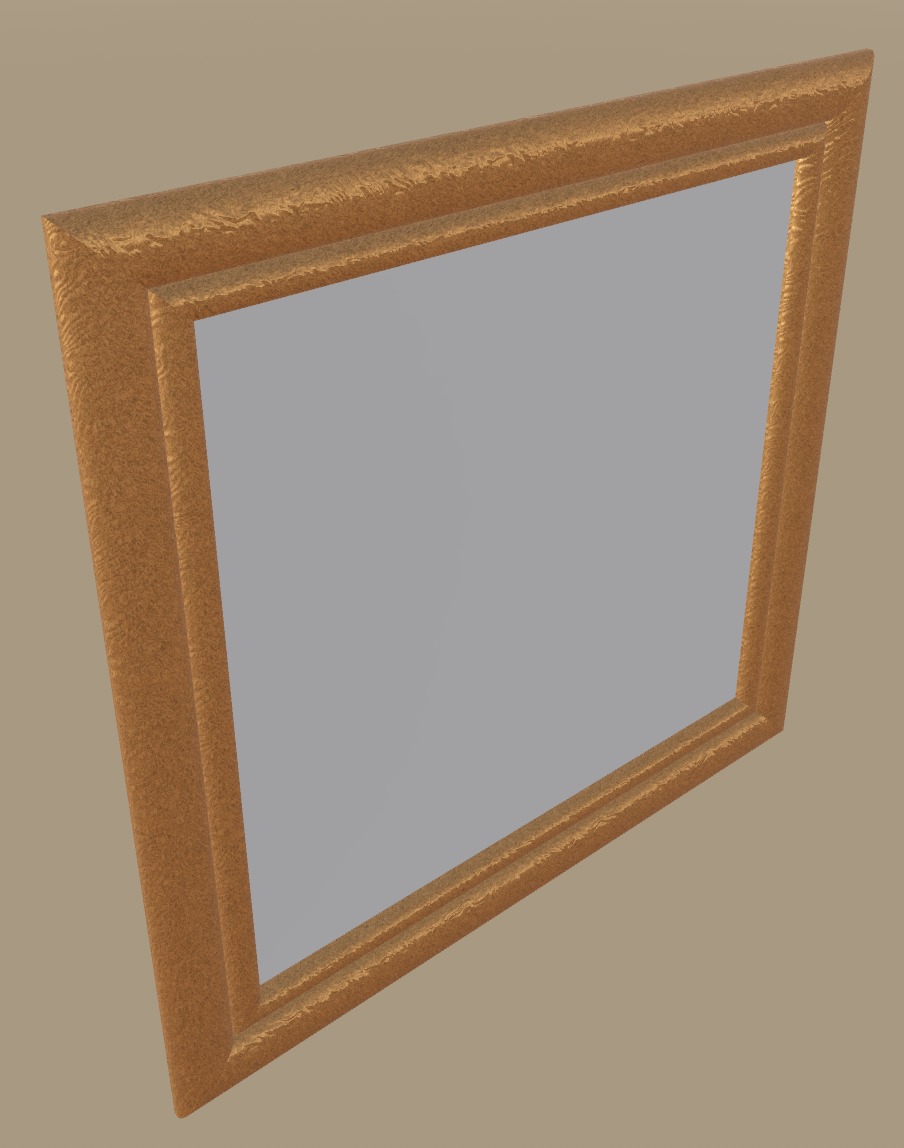
\includegraphics[height=3.12cm,keepaspectratio]{../Report/Figures/ch04-04-2d-frame.png}

    \vspace{0.08cm}
    \textcolor{unired}{\large\bfseries 2D EXHIBIT}

    \vspace{0.07cm}
    \footnotesize
    Adaptive frame and video playback.
  \end{column}
  \begin{column}{0.48\textwidth}
    \centering
    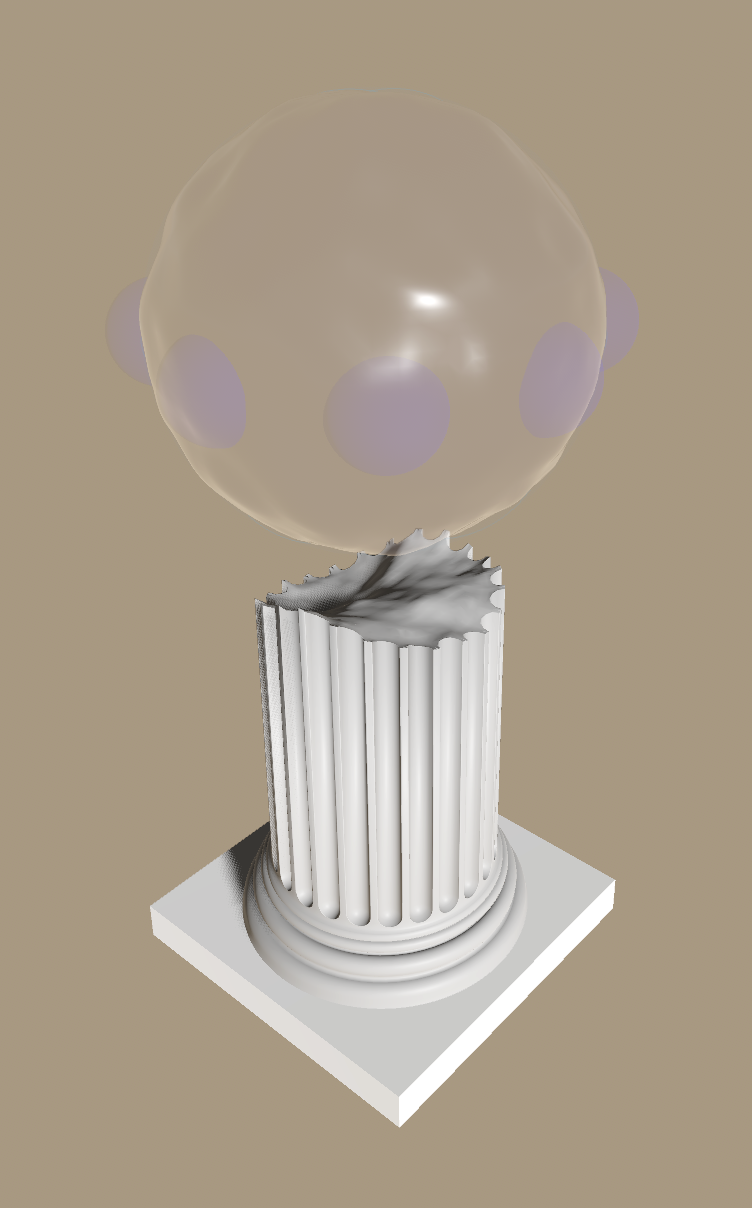
\includegraphics[height=3.12cm,keepaspectratio]{../Report/Figures/ch04-05-3d-orb-pillar.png}

    \vspace{0.08cm}
    \textcolor{unired}{\large\bfseries 3D EXHIBIT}

    \vspace{0.07cm}
    \footnotesize
    Fit, rotate and inspect in a separate room.
  \end{column}
\end{columns}

\vspace{0.18cm}
\begin{beamercolorbox}[sep=0.48em,rounded=true]{palette highlight}
  \centering\small
  Each exhibit carries the vector for \emph{Similar}.
\end{beamercolorbox}
\end{frame}
